\section{Introduction}
\label{sec:intro}

Datacenters, and the cloud, are at the center of today's storage needs.
While security is an utmost concern in these environments,
unfortunately, modern encrypted file systems do not match the needs
of today's users.  
We use systems like Dropbox to store, sync, and
share our files, but few existing encryption schemes support this
usage. Cloud storage systems like Amazon S3 are in
growing demand, but encrypting files stored on such system while also
allowing access at a variety of end points is a major challenge. Many
of our modern (and legacy) computing services, that are being migrated
to public and private clouds, are designed to run in
the background, devoid of interactive input.  Yet, most existing
encryption solutions require interactive input in order to securely
access encrypted files. 

The inability of existing encryption systems
to accommodate the diverse range of use cases we require leads to such
system being largely unusable. This inflexibility is not due to the
underlying encryption itself, but to the methods by which encryption
keys are managed and stored. Today, most file encryption solutions
tightly couple key storage with the underlying encryption. This is a
mistake that has lead to a growing usability gap and the corresponding
underutilization of encryption as a tool for securing and controlling
our data \cite{Whitten1999, Sweikata2009, Kher2005, Geambasu2011}, and
will carry over to the datacenter and cloud infrastructure.

We propose separating key storage and access management from the
underlying encryption scheme through a ``Key Storage as a Service''
system. Such a service makes encryption systems far more flexible and
accommodating of the diversity of modern use cases, and by extension
makes file encryption far easier to use. Strong encryption is one of
the best available tools for securing and protecting our data. We wish
to reclaim it as a viable option for controlling our data in
environments that are increasingly outside of our control.

%\begin{figure}[!tb]
%  \centering
%  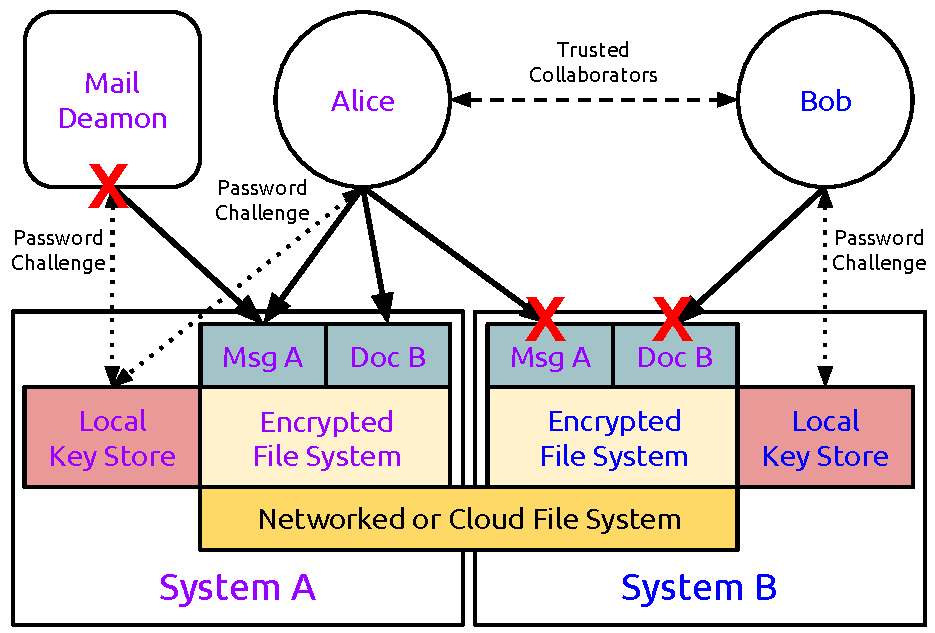
\includegraphics[width=\columnwidth]{./include/Problem-Layered.pdf}
%  \caption{Existing Local Encrypted File Systems}
%  \label{fig:problem-layered}
%\end{figure}

%As shown in Figure~\ref{fig:problem-layered}, 
Existing local encrypted file system solutions like
dm-crypt~\cite{dm-crypt} and eCryptfs~\cite{Halcrow} suffer from a
number of limitations related to their tightly-coupled local key
storage and access management components. These systems work fine for an
individual user like Alice wishing to secure file like her mail or
documents and access them from a single machine. But they quickly
break down when trying to move beyond the simple single-user,
single-device use case. Alice can not access her encrypted mail file
across a networked file system from System B since System B has no
access to the encryption keys stored on System A. Furthermore, she can
not share a work document with a trusted collaborator like Bob,
since Bob neither has access to her encryption keys stored on System A
nor the password required to unlock these keys. A non-interactive
process like the Mail Daemon is also unable to leverage these
encrypted file systems due to the inability of such services to
securely and interactively provide a password to unlock the keys
needed to decrypt local files.

%\begin{figure}[!tb]
%  \centering
%  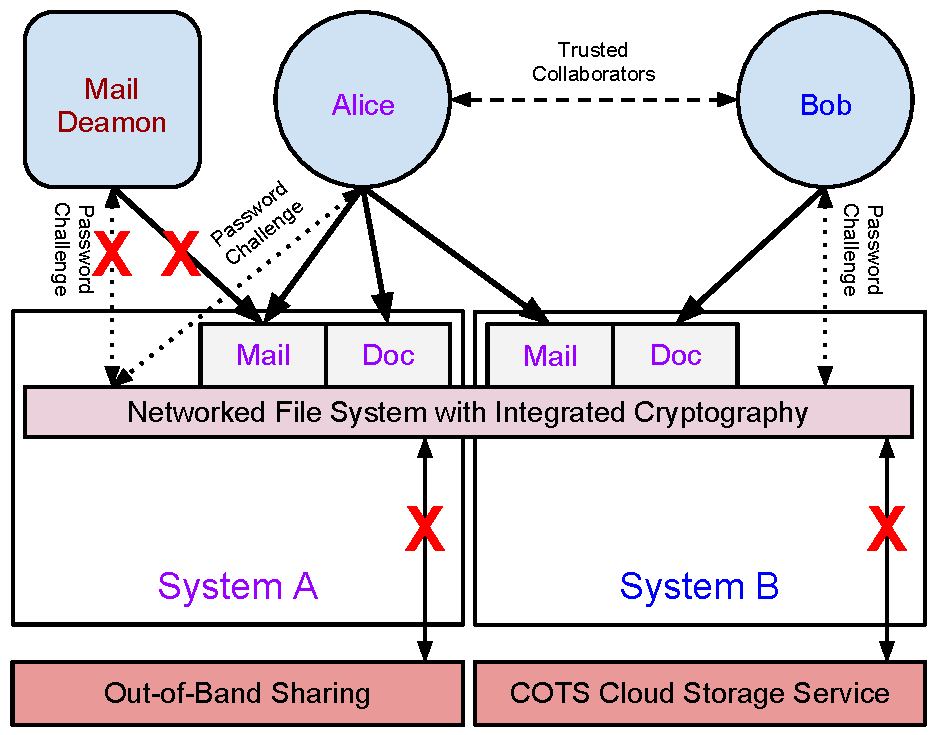
\includegraphics[width=\columnwidth]{./include/Problem-Integrated.pdf}
%  \caption{Existing Distributed Encrypted File Systems}
%  \label{fig:problem-integrated}
%\end{figure}

While distributed encrypted file systems such as
OceanStore~\cite{Kubiatowicz2000} or Tahoe~\cite{Wilcox-O'Hearn2008}
tend to succeed in solving some of the sharing and distribution
problems inherent in local secure file systems, they still lack the
flexibility required to address the full range of desired use
cases. 
%Figure \ref{fig:problem-integrated} shows some of the remaining
%issues inherent in distributed solutions. 
Notably, while multi-user
use cases are better supported, non-interactive use cases are still a
challenge. Furthermore, full stack distributed file systems tend to be
wedded with specific storage systems and thus lack support for
Cloud-based Storage as a Service offerings or alternate file system
technologies. These systems also lack support for most forms of
``out-of-band'' file sharing (via e-mail, USB flash drives, etc) due
to the inability of actors outside of the integrated stack to access
the necessary encryption keys.

Existing systems force the user into a very specific security model,
appropriate for certain use cases, but useless for many others. 
The cloud model enables services supporting a variety of needs 
rather than fixing a single use model.

In this proposal, we propose Custos (Figure~\ref{fig:custosoverview}), 
a flexible ``Key Storage as
a Service'' system designed to support a variety of data security
requirements across a wide range of use cases. 

\begin{figure}[!tb]
  \centering
  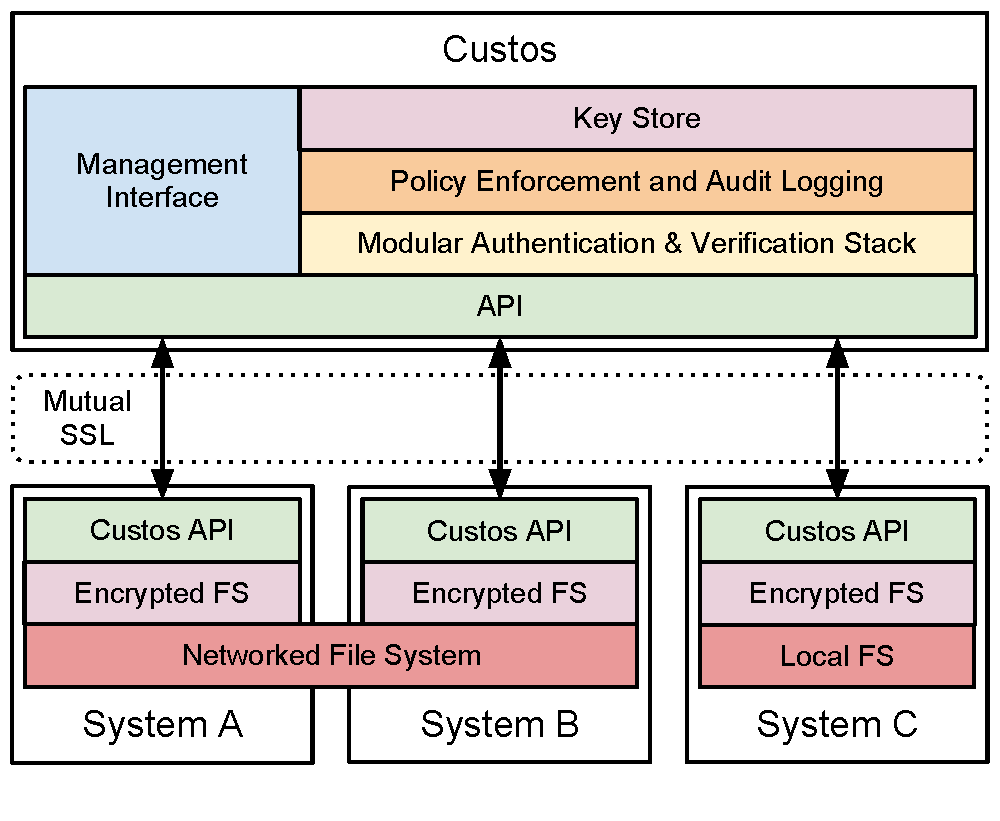
\includegraphics[width=\columnwidth]{./include/CustosOverview.pdf}
  \caption{Custos Architecture Overview}
  \label{fig:custosoverview}
\end{figure}

Custos is based on three core principles:

\noindent
\textbf{Decoupled Key Storage:}
Existing encryption systems almost always bundle their own key storage
and access control components. This practice unnecessarily couples the
authentication and authorization models used to protect encrypted
files with the actual encryption itself. 
Custos breaks this unnecessary coupling by providing a service to store the keys
required to encrypt or decrypt specific files, and to control who may
access each key. Custos exposes a key access API that provides a
standardized interface through which a variety of file encryption
systems may read, write, add, or delete keys. This allows Custos to
focus on key storage and access management, while individual
encryption systems focus the actual file encryption. Key storage and
access control is a fundamentally different problem than file
encryption, and as such it requires a fundamentally separate
service-oriented solution.


\noindent
\textbf{Flexible Security Models:}
Not all data is equal, and neither is the means with which we must
protect it. Any data
encryption system that forces a single authentication model on all
data it is designed to protect is inherently limiting.
Custos strives to overcome this issue by providing a flexible and
extensible authentication and requirements framework capable of
supporting separate access and threat models for each individual
file. 

\noindent
\textbf{Global Access and Centralization:}
The modern Internet not only allows us to move and share data at
levels never before possible, in many instances it requires it. Data
is no longer limited to a single machine, or even a single user, or single
organization. It is highly mobile and often shared (e.g., between users and between
services that a given user uses). The key storage and access control mechanisms
built into existing encryption system are not good at dealing with
this lose model of data location or access domain.
Custos addresses these issues via its design as a logically
centralized, globally accessible service.



\section{Relation to VMWare}

VMWare's product range extends far beyond virtualization technology.
The security of the hypervisor has been studied by researchers and 
industry alike.  The security of the
network has received attention, and with the acquisition of Nicira and 
the use of software-defined networking, VMWare is well positioned to
isolate tenants.  We argue that enabling technology for encrypted file systems,
beyond the encryption technology itself, has received little attention.
Custos would be a great compliment to products such as vSphere Storage 
Appliance.  In supporting this proposal, VMWare will be supporting 
the research behind Custos, including the building of Custos and 
more fully studying the variety of security models that will be
needed.  With collaboration with VMWare, we will gain invaluable 
insight into these security models.
